\documentclass[a4paper,10pt]{article}
\usepackage[pdftex]{color,graphicx}
\usepackage[pdftex, bookmarks, colorlinks=false]{hyperref}
\usepackage{longtable}
%\usepackage[all]{xy}
\addtolength{\textheight}{4cm}
\addtolength{\textwidth}{3cm}
\addtolength{\hoffset}{-3cm}
\addtolength{\voffset}{-3cm}

%opening
\title{Stuff casted out of paper}
\author{Yu Huang}

\begin{document}

\maketitle

\begin{abstract}
Here contains stuff not included in the official paper or trial and failure.
\end{abstract}

\tableofcontents

\section{Identity}

\subsection{2007-10-21 thinning the identity pairs by removing ambiguous NA-rich strains}
To enable component to reach transivity (true haplotype), magnus suggested a thinning algorithm.

Sort the individuals so that those with the smallest numbers of NA come on top.  Go through the individuals one at a time: if an individual is different (has a mismatch, ignoring NA) from one you have seen, add it to the list of unique haplotypes.

Given the list of unique haplotypes. Now go through the remainder and assign those that can be assigned uniquely (no mismatches).  Leave the ones that cannot be assigned uniquely unassigned.

this is a greedy algorithm, which can't gaurantee the transivity. (another algorithm is on the way to settle this...)

the number of identity pairs dropped to 364801 (15\% less) but the inter population identities percentage, 244826/364801=0.67112206381 is almost same as before.

Figure~\ref{f28} is the identity map after thinning. global pattern is still there. and two cross-ocean components are still there (data not shown).

\begin{figure}
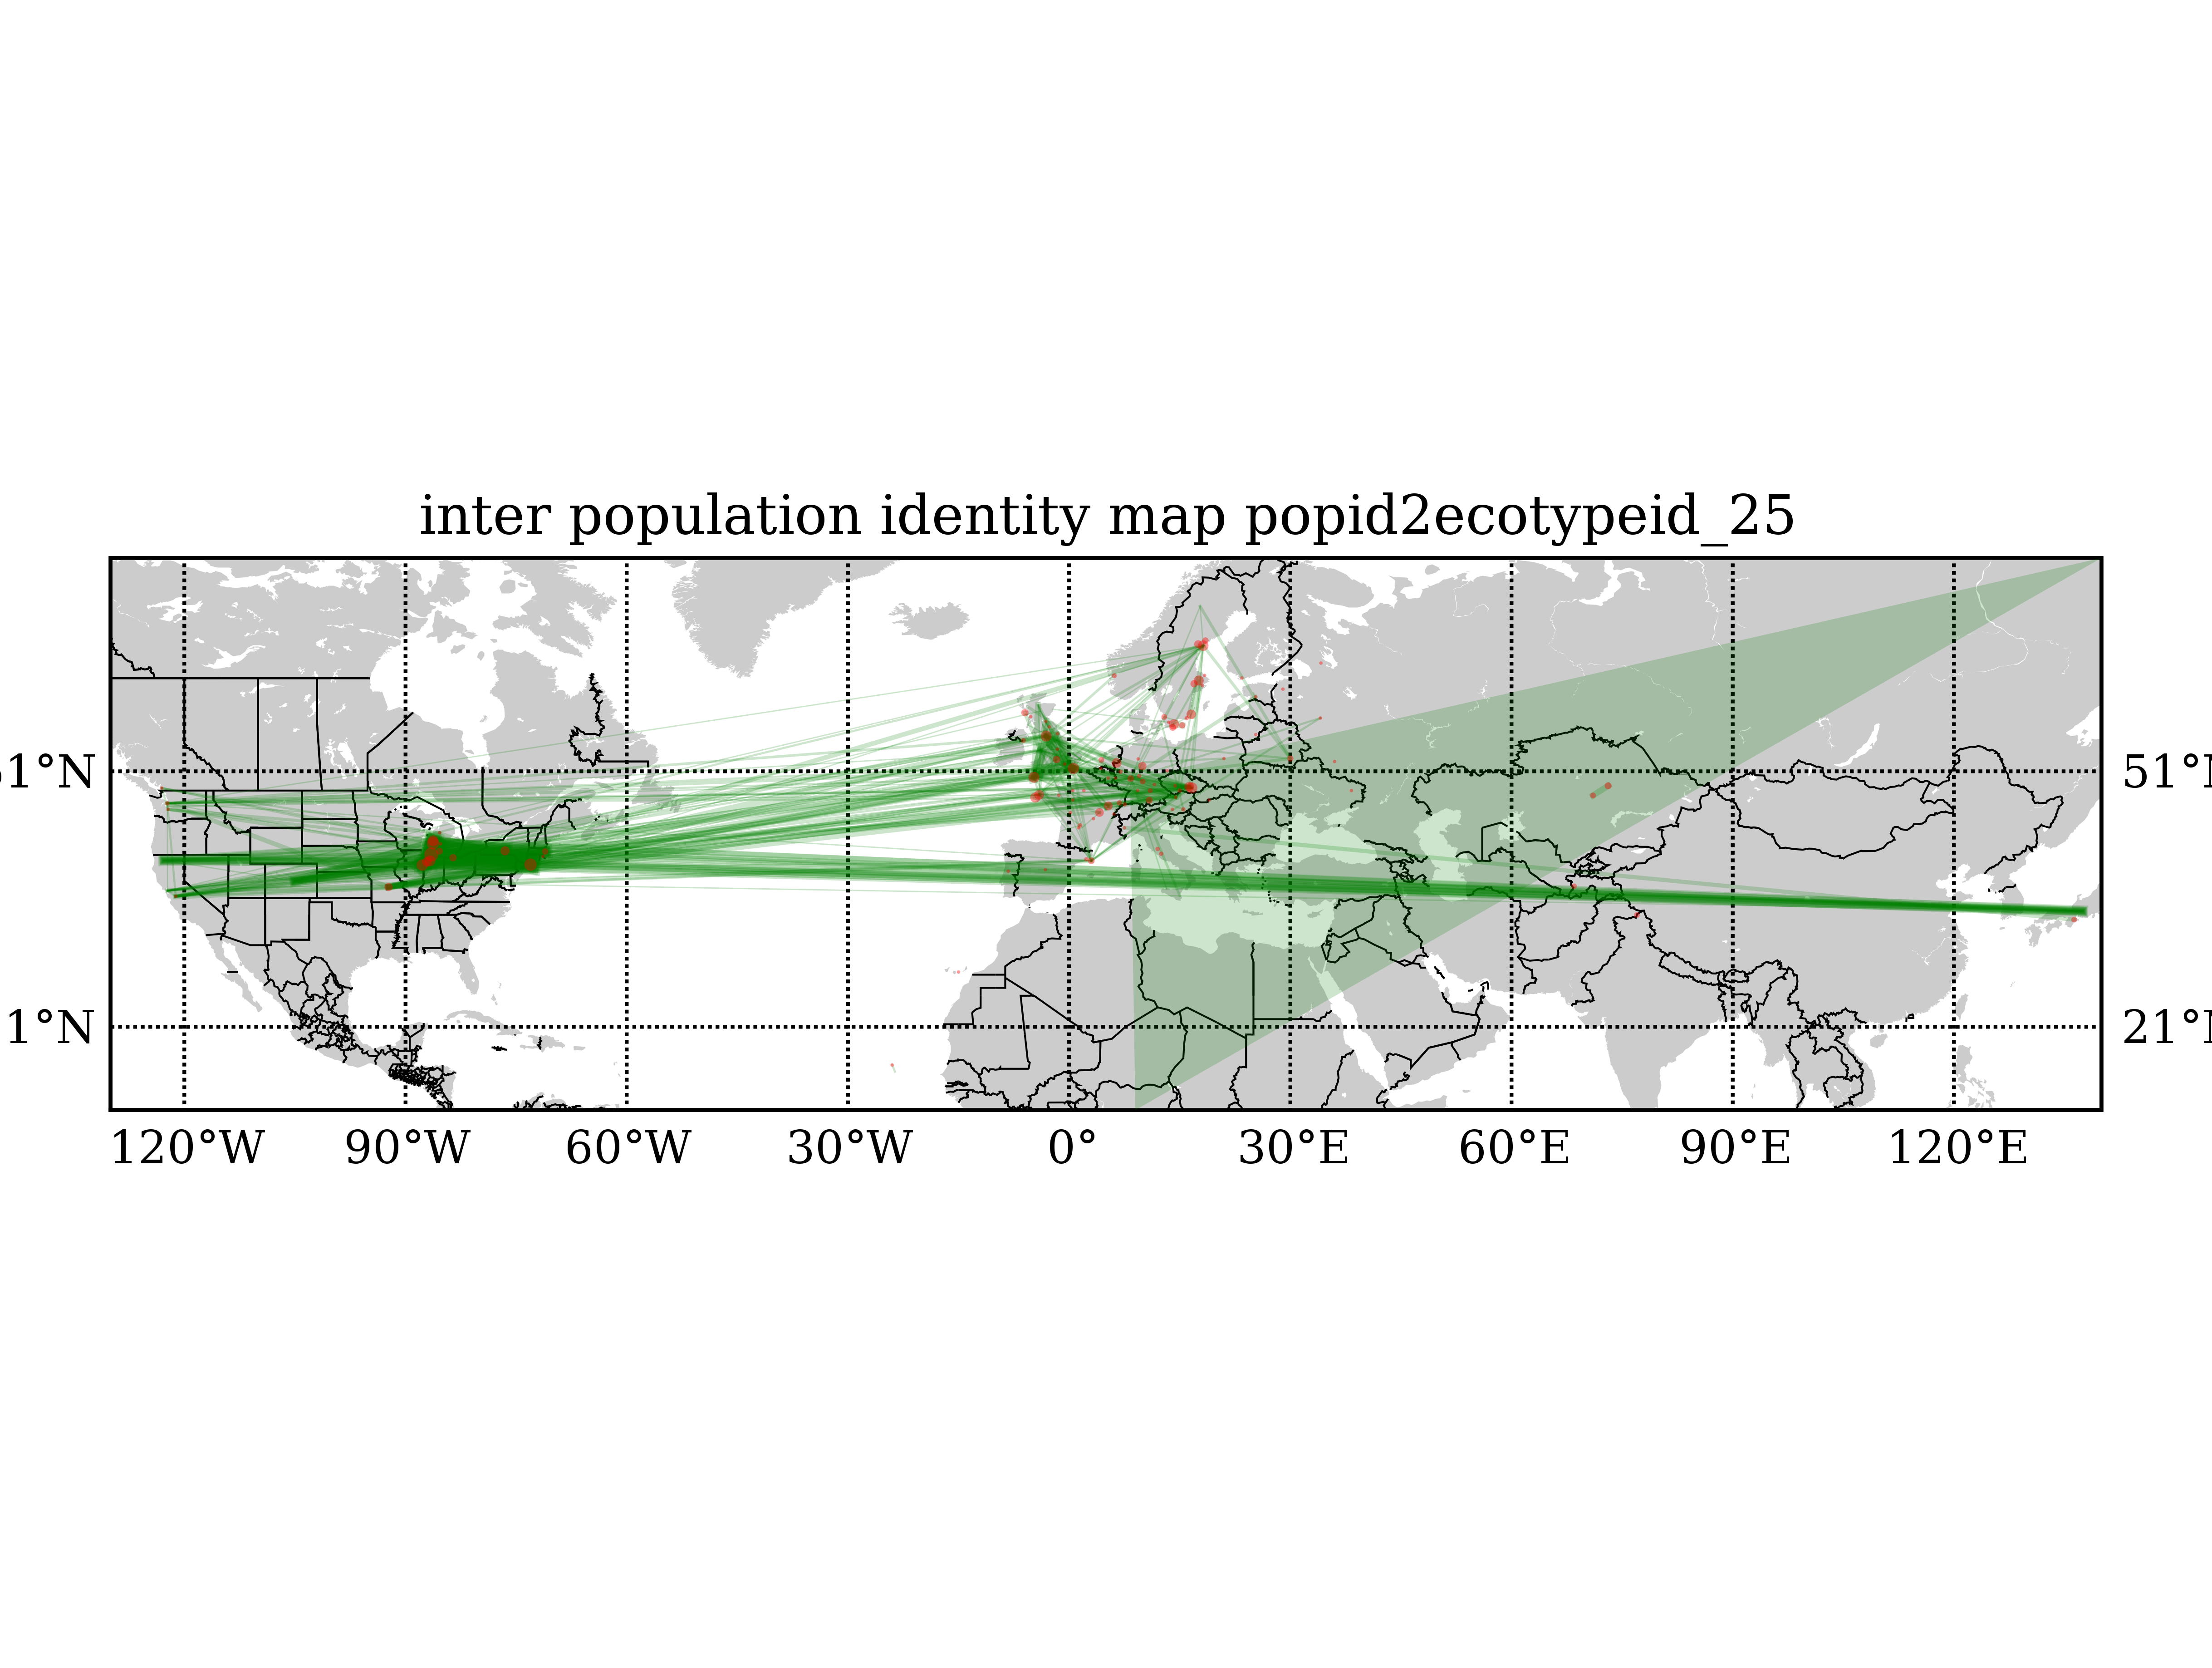
\includegraphics[width=1\textwidth]{figures/identity_map2_complete_site_network.png}
\caption{Population Identity Map after thinning}\label{f28}
\end{figure}

\end{document}
